\documentclass[12pt,a4paper]{article}
\usepackage[utf8]{vietnam}
\usepackage{amsmath,amssymb}
\usepackage{tabularx}
\usepackage{tikz}
\usepackage{xcolor}
\usepackage[top=0.6cm, bottom=0.6cm, left=0.6cm, right=0.6cm]{geometry}
\usepackage[dethi]{ex_test}

\SAOPTN{widthSA=3.2,heightSA=0.62}
\setlength{\parskip}{0pt}

% Dong ke cham mo chuan viet tay
\newcommand{\dongke}[1]{%
  \begingroup%
  \setlength{\parskip}{0pt}%
  \baselineskip=18.5pt%
  \vspace{1.0mm}%
  \foreach \i in {1,...,#1}{%
    \noindent{\color{gray!60}\dotfill}\par%
  }%
  \vspace{0.6mm}%
  \endgroup%
}

% Dinh nghia o bai tap tu luan trong bang
\newcommand{\oBaiTap}[3][6]{%
  \vspace{1.0mm}%
  \noindent\textbf{#2} #3\par%
  \dongke{#1}%
}

\begin{document}
\pagestyle{empty}
% =============================================================================
% ========================= TOAN 9 TUAN 09 BUOI 01 - MA DE 101 =================
% ========================= TRANG 1/2 ==========================================
% =============================================================================
\noindent
\begin{tabularx}{\linewidth}{|X|c|}
\hline
\textbf{PHIẾU KIỂM TRA ĐỊNH KỲ TOÁN 9 - TUẦN 09 - BUỔI 01} & \textbf{Mã đề: 101 - Trang 1/2} \\
\hline
\end{tabularx}

\vspace{1.0mm}

\noindent
\begin{tabularx}{\linewidth}{|p{3.2cm}|X|}
\hline
\centering\textbf{ĐIỂM SỐ} & \centering\textbf{LỜI NHẬN XÉT CỦA THẦY CÔ} \tabularnewline
\hline
\rule{0pt}{1.8cm} & \tabularnewline
\hline
\end{tabularx}

\vspace{1.2mm}
\noindent\textbf{Câu 1 (0,25 điểm).} Cho đường tròn $(O; 5\text{ cm})$. Điểm $M$ có $OM = 4\text{ cm}$. Vị trí của $M$ là: \shortans{Nằm trong}\par\vspace{0.6mm}
\noindent\textbf{Câu 2 (0,25 điểm).} Tâm của đường tròn ngoại tiếp tam giác vuông là điểm nào?: \shortans{Trung điểm cạnh huyền}\par\vspace{0.6mm}
\noindent\textbf{Câu 3 (0,25 điểm).} Dây lớn nhất của một đường tròn là đoạn thẳng nào?: \shortans{Đường kính}\par\vspace{0.6mm}
\noindent\textbf{Câu 4 (0,25 điểm).} Căn bậc hai số học của số $49$ là: \shortans{7}\par\vspace{0.6mm}
\noindent\textbf{Câu 5 (0,25 điểm).} Điều kiện xác định của biểu thức $\sqrt{2x - 6}$ là: \shortans{x \ge 3}\par\vspace{0.6mm}
\noindent\textbf{Câu 6 (0,25 điểm).} Kết quả rút gọn biểu thức $\sqrt{18} - \sqrt{8} + \sqrt{2}$ bằng: \shortans{2\sqrt{2}}\par\vspace{0.6mm}
\noindent\textbf{Câu 7 (0,25 điểm).} Nghiệm của hệ phương trình $\begin{cases} x + y = 5 \\ x - y = 1 \end{cases}$ là $(x; y) = $: \shortans{(3; 2)}\par\vspace{0.6mm}
\noindent\textbf{Câu 8 (0,25 điểm).} Tam giác vuông có cạnh đối bằng $3$, cạnh huyền bằng $5$. Sin góc đối là: \shortans{\dfrac{3}{5}}\par\vspace{0.6mm}
\noindent\textbf{Câu 9 (0,25 điểm).} Tam giác vuông có hai cạnh góc vuông $6\text{ cm}, 8\text{ cm}$. Bán kính ngoại tiếp là: \shortans{5\text{ cm}}\par\vspace{0.6mm}
\noindent\textbf{Câu 10 (0,25 điểm).} Trạm phát sóng có bán kính $15\text{ km}$, máy cách $12\text{ km}$ có nhận được sóng không?: \shortans{Có}\par\vspace{0.6mm}
\vspace{0.8mm}
\noindent\textbf{Câu 11 (2,5 điểm). Đại số tổng hợp:}
\vspace{0.6mm}

\noindent
\begin{tabularx}{\linewidth}{|X|X|}
\hline
\oBaiTap[19]{a) (1,25 điểm)}{Giải hệ phương trình:\par $\begin{cases} 2x + y = 8 \\ 3x - y = 7 \end{cases}$} & 
\oBaiTap[19]{b) (1,25 điểm)}{Cho $P = \left(\dfrac{\sqrt{x}}{\sqrt{x}+2} + \dfrac{4\sqrt{x}}{x-4}\right) : \dfrac{\sqrt{x}+2}{x-4}$ với $x > 0, x \ne 4$.\par Rút gọn $P$ và tính giá trị của $P$ tại $x = 9$.} \\
\hline
\end{tabularx}

\newpage
% =============================================================================
% ========================= TOAN 9 TUAN 09 BUOI 01 - MA DE 101 =================
% ========================= TRANG 2/2 ==========================================
% =============================================================================
\noindent
\begin{tabularx}{\linewidth}{|X|c|}
\hline
\textbf{TOÁN 9 - TUẦN 09 - BUỔI 01} & \textbf{Mã đề: 101 - Trang 2/2} \\
\hline
\end{tabularx}

\vspace{1.2mm}

\noindent
\begin{tabularx}{\linewidth}{|X|}
\hline
\vspace{0.5mm}
\textbf{Câu 12 (2,5 điểm).} Theo kế hoạch, hai tổ sản xuất phải làm được tổng cộng $600$ sản phẩm. Nhờ cải tiến kỹ thuật, tổ I đã làm vượt mức kế hoạch $15\%$, tổ II đã làm vượt mức kế hoạch $20\%$, do đó cả hai tổ đã làm được $705$ sản phẩm. Hỏi theo kế hoạch, mỗi tổ phải sản xuất bao nhiêu sản phẩm?\par
\vspace{0.4mm}
\noindent\textit{Bài giải:}\dongke{16}
\\ \hline
\end{tabularx}

\vspace{1.5mm}

\noindent
\begin{tabularx}{\linewidth}{|X|}
\hline
\vspace{0.5mm}
\begin{minipage}[t]{0.64\linewidth}
\vspace{0pt}
\textbf{Câu 13 (2,5 điểm).} Cho tam giác $ABC$ nhọn ($AB < AC$), các đường cao $BD$ và $CE$ cắt nhau tại $H$ ($D \in AC, E \in AB$).\par\vspace{0.4mm}
\textbf{a) (1,25 điểm)} Chứng minh $4$ điểm $B, E, D, C$ cùng thuộc một đường tròn. Xác định tâm và bán kính của đường tròn đó.\par\vspace{0.4mm}
\textbf{b) (1,25 điểm)} Chứng minh $4$ điểm $A, E, H, D$ cùng thuộc một đường tròn. Xác định tâm của đường tròn đó.
\end{minipage}\hfill
\begin{minipage}[t]{0.34\linewidth}
\vspace{0pt}\centering
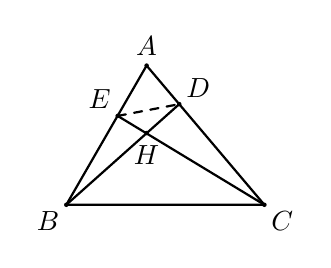
\begin{tikzpicture}[scale=0.68, >=stealth, line join=round, line cap=round]
  \coordinate (A) at (0, 2.6);
  \coordinate (B) at (-1.5, 0);
  \coordinate (C) at (2.2, 0);
  \coordinate (D) at (0.61, 1.88);
  \coordinate (E) at (-0.54, 1.66);
  \coordinate (H) at (0, 1.34);
  \draw[thick] (A) -- (B) -- (C) -- cycle;
  \draw[thick] (B) -- (D);
  \draw[thick] (C) -- (E);
  \draw[thick, dashed] (E) -- (D);
  \fill (A) circle (1.2pt) node[above] {$A$};
  \fill (B) circle (1.2pt) node[below left=-1pt] {$B$};
  \fill (C) circle (1.2pt) node[below right=-1pt] {$C$};
  \fill (D) circle (1.2pt) node[above right=-1pt] {$D$};
  \fill (E) circle (1.2pt) node[above left=-1pt] {$E$};
  \fill (H) circle (1.2pt) node[below=1pt] {$H$};
\end{tikzpicture}
\end{minipage}\par
\vspace{0.4mm}
\noindent\textit{Bài giải:}\dongke{17}
\\ \hline
\end{tabularx}

\newpage
% =============================================================================
% ========================= TOAN 9 TUAN 09 BUOI 01 - MA DE 102 =================
% ========================= TRANG 1/2 ==========================================
% =============================================================================
\noindent
\begin{tabularx}{\linewidth}{|X|c|}
\hline
\textbf{PHIẾU KIỂM TRA ĐỊNH KỲ TOÁN 9 - TUẦN 09 - BUỔI 01} & \textbf{Mã đề: 102 - Trang 1/2} \\
\hline
\end{tabularx}

\vspace{1.0mm}

\noindent
\begin{tabularx}{\linewidth}{|p{3.2cm}|X|}
\hline
\centering\textbf{ĐIỂM SỐ} & \centering\textbf{LỜI NHẬN XÉT CỦA THẦY CÔ} \tabularnewline
\hline
\rule{0pt}{1.8cm} & \tabularnewline
\hline
\end{tabularx}

\vspace{1.2mm}
\noindent\textbf{Câu 1 (0,25 điểm).} Cho đường tròn $(O; 5\text{ cm})$. Điểm $M$ có $OM = 5\text{ cm}$. Vị trí của $M$ là: \shortans{Nằm trên}\par\vspace{0.6mm}
\noindent\textbf{Câu 2 (0,25 điểm).} Tam giác $ABC$ vuông tại $A$ có $BC = 10\text{ cm}$. Bán kính ngoại tiếp là: \shortans{5\text{ cm}}\par\vspace{0.6mm}
\noindent\textbf{Câu 3 (0,25 điểm).} Đường tròn $(O; 4\text{ cm})$ có dây lớn nhất dài bao nhiêu?: \shortans{8\text{ cm}}\par\vspace{0.6mm}
\noindent\textbf{Câu 4 (0,25 điểm).} Căn bậc hai số học của số $64$ là: \shortans{8}\par\vspace{0.6mm}
\noindent\textbf{Câu 5 (0,25 điểm).} Điều kiện xác định của biểu thức $\sqrt{3x - 12}$ là: \shortans{x \ge 4}\par\vspace{0.6mm}
\noindent\textbf{Câu 6 (0,25 điểm).} Kết quả rút gọn biểu thức $\sqrt{27} - \sqrt{12} + \sqrt{3}$ bằng: \shortans{2\sqrt{3}}\par\vspace{0.6mm}
\noindent\textbf{Câu 7 (0,25 điểm).} Nghiệm của hệ phương trình $\begin{cases} x + y = 6 \\ x - y = 2 \end{cases}$ là $(x; y) = $: \shortans{(4; 2)}\par\vspace{0.6mm}
\noindent\textbf{Câu 8 (0,25 điểm).} Tam giác vuông có cạnh kề bằng $4$, cạnh huyền bằng $5$. Cos góc kề là: \shortans{\dfrac{4}{5}}\par\vspace{0.6mm}
\noindent\textbf{Câu 9 (0,25 điểm).} Tam giác vuông có hai cạnh góc vuông $5\text{ cm}, 12\text{ cm}$. Bán kính ngoại tiếp là: \shortans{6{,}5\text{ cm}}\par\vspace{0.6mm}
\noindent\textbf{Câu 10 (0,25 điểm).} Trạm phát sóng có bán kính $20\text{ km}$, máy cách $22\text{ km}$ có nhận được sóng không?: \shortans{Không}\par\vspace{0.6mm}
\vspace{0.8mm}
\noindent\textbf{Câu 11 (2,5 điểm). Đại số tổng hợp:}
\vspace{0.6mm}

\noindent
\begin{tabularx}{\linewidth}{|X|X|}
\hline
\oBaiTap[19]{a) (1,25 điểm)}{Giải hệ phương trình:\par $\begin{cases} 3x + y = 11 \\ 2x - y = 4 \end{cases}$} & 
\oBaiTap[19]{b) (1,25 điểm)}{Cho $P = \left(\dfrac{\sqrt{x}}{\sqrt{x}+3} + \dfrac{6\sqrt{x}}{x-9}\right) : \dfrac{\sqrt{x}+3}{x-9}$ với $x > 0, x \ne 9$.\par Rút gọn $P$ và tính giá trị của $P$ tại $x = 16$.} \\
\hline
\end{tabularx}

\newpage
% =============================================================================
% ========================= TOAN 9 TUAN 09 BUOI 01 - MA DE 102 =================
% ========================= TRANG 2/2 ==========================================
% =============================================================================
\noindent
\begin{tabularx}{\linewidth}{|X|c|}
\hline
\textbf{TOÁN 9 - TUẦN 09 - BUỔI 01} & \textbf{Mã đề: 102 - Trang 2/2} \\
\hline
\end{tabularx}

\vspace{1.2mm}

\noindent
\begin{tabularx}{\linewidth}{|X|}
\hline
\vspace{0.5mm}
\textbf{Câu 12 (2,5 điểm).} Theo kế hoạch, hai tổ công nhân dự định dệt tổng cộng $700$ chiếc áo len. Do thi đua, tổ I dệt vượt mức $10\%$, tổ II dệt vượt mức $15\%$, nên cả hai tổ đã dệt được $785$ chiếc áo len. Hỏi theo kế hoạch, mỗi tổ dự định dệt bao nhiêu chiếc áo len?\par
\vspace{0.4mm}
\noindent\textit{Bài giải:}\dongke{16}
\\ \hline
\end{tabularx}

\vspace{1.5mm}

\noindent
\begin{tabularx}{\linewidth}{|X|}
\hline
\vspace{0.5mm}
\begin{minipage}[t]{0.64\linewidth}
\vspace{0pt}
\textbf{Câu 13 (2,5 điểm).} Cho tam giác $ABC$ nhọn ($AB < AC$), các đường cao $BD$ và $CE$ cắt nhau tại $H$ ($D \in AC, E \in AB$).\par\vspace{0.4mm}
\textbf{a) (1,25 điểm)} Chứng minh $4$ điểm $B, E, D, C$ cùng thuộc một đường tròn. Xác định tâm và bán kính của đường tròn đó.\par\vspace{0.4mm}
\textbf{b) (1,25 điểm)} Chứng minh $4$ điểm $A, E, H, D$ cùng thuộc một đường tròn. Xác định tâm của đường tròn đó.
\end{minipage}\hfill
\begin{minipage}[t]{0.34\linewidth}
\vspace{0pt}\centering
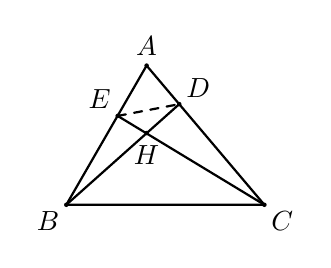
\begin{tikzpicture}[scale=0.68, >=stealth, line join=round, line cap=round]
  \coordinate (A) at (0, 2.6);
  \coordinate (B) at (-1.5, 0);
  \coordinate (C) at (2.2, 0);
  \coordinate (D) at (0.61, 1.88);
  \coordinate (E) at (-0.54, 1.66);
  \coordinate (H) at (0, 1.34);
  \draw[thick] (A) -- (B) -- (C) -- cycle;
  \draw[thick] (B) -- (D);
  \draw[thick] (C) -- (E);
  \draw[thick, dashed] (E) -- (D);
  \fill (A) circle (1.2pt) node[above] {$A$};
  \fill (B) circle (1.2pt) node[below left=-1pt] {$B$};
  \fill (C) circle (1.2pt) node[below right=-1pt] {$C$};
  \fill (D) circle (1.2pt) node[above right=-1pt] {$D$};
  \fill (E) circle (1.2pt) node[above left=-1pt] {$E$};
  \fill (H) circle (1.2pt) node[below=1pt] {$H$};
\end{tikzpicture}
\end{minipage}\par
\vspace{0.4mm}
\noindent\textit{Bài giải:}\dongke{17}
\\ \hline
\end{tabularx}

\newpage
% =============================================================================
% ========================= TOAN 9 TUAN 09 BUOI 01 - MA DE 103 =================
% ========================= TRANG 1/2 ==========================================
% =============================================================================
\noindent
\begin{tabularx}{\linewidth}{|X|c|}
\hline
\textbf{PHIẾU KIỂM TRA ĐỊNH KỲ TOÁN 9 - TUẦN 09 - BUỔI 01} & \textbf{Mã đề: 103 - Trang 1/2} \\
\hline
\end{tabularx}

\vspace{1.0mm}

\noindent
\begin{tabularx}{\linewidth}{|p{3.2cm}|X|}
\hline
\centering\textbf{ĐIỂM SỐ} & \centering\textbf{LỜI NHẬN XÉT CỦA THẦY CÔ} \tabularnewline
\hline
\rule{0pt}{1.8cm} & \tabularnewline
\hline
\end{tabularx}

\vspace{1.2mm}
\noindent\textbf{Câu 1 (0,25 điểm).} Cho đường tròn $(O; 5\text{ cm})$. Điểm $M$ có $OM = 6\text{ cm}$. Vị trí của $M$ là: \shortans{Nằm ngoài}\par\vspace{0.6mm}
\noindent\textbf{Câu 2 (0,25 điểm).} Tam giác $ABC$ vuông tại $A$ có $BC = 12\text{ cm}$. Bán kính ngoại tiếp là: \shortans{6\text{ cm}}\par\vspace{0.6mm}
\noindent\textbf{Câu 3 (0,25 điểm).} Đường tròn $(O; 6\text{ cm})$ có dây lớn nhất dài bao nhiêu?: \shortans{12\text{ cm}}\par\vspace{0.6mm}
\noindent\textbf{Câu 4 (0,25 điểm).} Căn bậc hai số học của số $81$ là: \shortans{9}\par\vspace{0.6mm}
\noindent\textbf{Câu 5 (0,25 điểm).} Điều kiện xác định của biểu thức $\sqrt{4x - 8}$ là: \shortans{x \ge 2}\par\vspace{0.6mm}
\noindent\textbf{Câu 6 (0,25 điểm).} Kết quả rút gọn biểu thức $\sqrt{50} - \sqrt{18} + \sqrt{2}$ bằng: \shortans{3\sqrt{2}}\par\vspace{0.6mm}
\noindent\textbf{Câu 7 (0,25 điểm).} Nghiệm của hệ phương trình $\begin{cases} x + y = 7 \\ x - y = 3 \end{cases}$ là $(x; y) = $: \shortans{(5; 2)}\par\vspace{0.6mm}
\noindent\textbf{Câu 8 (0,25 điểm).} Tam giác vuông có cạnh đối bằng $5$, cạnh huyền bằng $13$. Sin góc đối là: \shortans{\dfrac{5}{13}}\par\vspace{0.6mm}
\noindent\textbf{Câu 9 (0,25 điểm).} Tam giác vuông có hai cạnh góc vuông $8\text{ cm}, 15\text{ cm}$. Bán kính ngoại tiếp là: \shortans{8{,}5\text{ cm}}\par\vspace{0.6mm}
\noindent\textbf{Câu 10 (0,25 điểm).} Bánh xe có bán kính $0{,}3\text{ m}$. Đường kính của bánh xe là: \shortans{0{,}6\text{ m}}\par\vspace{0.6mm}
\vspace{0.8mm}
\noindent\textbf{Câu 11 (2,5 điểm). Đại số tổng hợp:}
\vspace{0.6mm}

\noindent
\begin{tabularx}{\linewidth}{|X|X|}
\hline
\oBaiTap[19]{a) (1,25 điểm)}{Giải hệ phương trình:\par $\begin{cases} 2x - y = 3 \\ 3x + y = 12 \end{cases}$} & 
\oBaiTap[19]{b) (1,25 điểm)}{Cho $P = \left(\dfrac{\sqrt{x}}{\sqrt{x}+1} + \dfrac{2\sqrt{x}}{x-1}\right) : \dfrac{\sqrt{x}+1}{x-1}$ với $x > 0, x \ne 1$.\par Rút gọn $P$ và tính giá trị của $P$ tại $x = 25$.} \\
\hline
\end{tabularx}

\newpage
% =============================================================================
% ========================= TOAN 9 TUAN 09 BUOI 01 - MA DE 103 =================
% ========================= TRANG 2/2 ==========================================
% =============================================================================
\noindent
\begin{tabularx}{\linewidth}{|X|c|}
\hline
\textbf{TOÁN 9 - TUẦN 09 - BUỔI 01} & \textbf{Mã đề: 103 - Trang 2/2} \\
\hline
\end{tabularx}

\vspace{1.2mm}

\noindent
\begin{tabularx}{\linewidth}{|X|}
\hline
\vspace{0.5mm}
\textbf{Câu 12 (2,5 điểm).} Theo kế hoạch, hai tổ may phải làm tổng cộng $800$ bộ quần áo. Nhờ thi đua, tổ I đã làm vượt mức kế hoạch $20\%$, tổ II làm vượt mức kế hoạch $15\%$, do đó cả hai tổ đã làm được $940$ bộ quần áo. Hỏi theo kế hoạch, mỗi tổ phải may bao nhiêu bộ quần áo?\par
\vspace{0.4mm}
\noindent\textit{Bài giải:}\dongke{16}
\\ \hline
\end{tabularx}

\vspace{1.5mm}

\noindent
\begin{tabularx}{\linewidth}{|X|}
\hline
\vspace{0.5mm}
\begin{minipage}[t]{0.64\linewidth}
\vspace{0pt}
\textbf{Câu 13 (2,5 điểm).} Cho tam giác $ABC$ nhọn ($AB < AC$), các đường cao $BD$ và $CE$ cắt nhau tại $H$ ($D \in AC, E \in AB$).\par\vspace{0.4mm}
\textbf{a) (1,25 điểm)} Chứng minh $4$ điểm $B, E, D, C$ cùng thuộc một đường tròn. Xác định tâm và bán kính của đường tròn đó.\par\vspace{0.4mm}
\textbf{b) (1,25 điểm)} Chứng minh $4$ điểm $A, E, H, D$ cùng thuộc một đường tròn. Xác định tâm của đường tròn đó.
\end{minipage}\hfill
\begin{minipage}[t]{0.34\linewidth}
\vspace{0pt}\centering
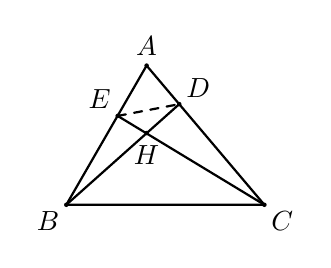
\begin{tikzpicture}[scale=0.68, >=stealth, line join=round, line cap=round]
  \coordinate (A) at (0, 2.6);
  \coordinate (B) at (-1.5, 0);
  \coordinate (C) at (2.2, 0);
  \coordinate (D) at (0.61, 1.88);
  \coordinate (E) at (-0.54, 1.66);
  \coordinate (H) at (0, 1.34);
  \draw[thick] (A) -- (B) -- (C) -- cycle;
  \draw[thick] (B) -- (D);
  \draw[thick] (C) -- (E);
  \draw[thick, dashed] (E) -- (D);
  \fill (A) circle (1.2pt) node[above] {$A$};
  \fill (B) circle (1.2pt) node[below left=-1pt] {$B$};
  \fill (C) circle (1.2pt) node[below right=-1pt] {$C$};
  \fill (D) circle (1.2pt) node[above right=-1pt] {$D$};
  \fill (E) circle (1.2pt) node[above left=-1pt] {$E$};
  \fill (H) circle (1.2pt) node[below=1pt] {$H$};
\end{tikzpicture}
\end{minipage}\par
\vspace{0.4mm}
\noindent\textit{Bài giải:}\dongke{17}
\\ \hline
\end{tabularx}

\newpage
% =============================================================================
% ========================= TOAN 9 TUAN 09 BUOI 01 - MA DE 104 =================
% ========================= TRANG 1/2 ==========================================
% =============================================================================
\noindent
\begin{tabularx}{\linewidth}{|X|c|}
\hline
\textbf{PHIẾU KIỂM TRA ĐỊNH KỲ TOÁN 9 - TUẦN 09 - BUỔI 01} & \textbf{Mã đề: 104 - Trang 1/2} \\
\hline
\end{tabularx}

\vspace{1.0mm}

\noindent
\begin{tabularx}{\linewidth}{|p{3.2cm}|X|}
\hline
\centering\textbf{ĐIỂM SỐ} & \centering\textbf{LỜI NHẬN XÉT CỦA THẦY CÔ} \tabularnewline
\hline
\rule{0pt}{1.8cm} & \tabularnewline
\hline
\end{tabularx}

\vspace{1.2mm}
\noindent\textbf{Câu 1 (0,25 điểm).} Cho đường tròn $(O; 6\text{ cm})$. Điểm $M$ có $OM = 4\text{ cm}$. Vị trí của $M$ là: \shortans{Nằm trong}\par\vspace{0.6mm}
\noindent\textbf{Câu 2 (0,25 điểm).} Tam giác $ABC$ vuông tại $A$ có $BC = 16\text{ cm}$. Bán kính ngoại tiếp là: \shortans{8\text{ cm}}\par\vspace{0.6mm}
\noindent\textbf{Câu 3 (0,25 điểm).} Đường tròn $(O; 5\text{ cm})$ có dây lớn nhất dài bao nhiêu?: \shortans{10\text{ cm}}\par\vspace{0.6mm}
\noindent\textbf{Câu 4 (0,25 điểm).} Căn bậc hai số học của số $100$ là: \shortans{10}\par\vspace{0.6mm}
\noindent\textbf{Câu 5 (0,25 điểm).} Điều kiện xác định của biểu thức $\sqrt{5x - 25}$ là: \shortans{x \ge 5}\par\vspace{0.6mm}
\noindent\textbf{Câu 6 (0,25 điểm).} Kết quả rút gọn biểu thức $\sqrt{75} - \sqrt{48} + \sqrt{3}$ bằng: \shortans{2\sqrt{3}}\par\vspace{0.6mm}
\noindent\textbf{Câu 7 (0,25 điểm).} Nghiệm của hệ phương trình $\begin{cases} x + y = 8 \\ x - y = 4 \end{cases}$ là $(x; y) = $: \shortans{(6; 2)}\par\vspace{0.6mm}
\noindent\textbf{Câu 8 (0,25 điểm).} Tam giác vuông có cạnh kề bằng $12$, cạnh huyền bằng $13$. Cos góc kề là: \shortans{\dfrac{12}{13}}\par\vspace{0.6mm}
\noindent\textbf{Câu 9 (0,25 điểm).} Tam giác vuông có hai cạnh góc vuông $9\text{ cm}, 12\text{ cm}$. Bán kính ngoại tiếp là: \shortans{7{,}5\text{ cm}}\par\vspace{0.6mm}
\noindent\textbf{Câu 10 (0,25 điểm).} Bánh xe có đường kính $70\text{ cm}$. Bán kính của bánh xe là: \shortans{35\text{ cm}}\par\vspace{0.6mm}
\vspace{0.8mm}
\noindent\textbf{Câu 11 (2,5 điểm). Đại số tổng hợp:}
\vspace{0.6mm}

\noindent
\begin{tabularx}{\linewidth}{|X|X|}
\hline
\oBaiTap[19]{a) (1,25 điểm)}{Giải hệ phương trình:\par $\begin{cases} 3x - y = 7 \\ 2x + y = 8 \end{cases}$} & 
\oBaiTap[19]{b) (1,25 điểm)}{Cho $P = \left(\dfrac{\sqrt{x}}{\sqrt{x}+4} + \dfrac{8\sqrt{x}}{x-16}\right) : \dfrac{\sqrt{x}+4}{x-16}$ với $x > 0, x \ne 16$.\par Rút gọn $P$ và tính giá trị của $P$ tại $x = 9$.} \\
\hline
\end{tabularx}

\newpage
% =============================================================================
% ========================= TOAN 9 TUAN 09 BUOI 01 - MA DE 104 =================
% ========================= TRANG 2/2 ==========================================
% =============================================================================
\noindent
\begin{tabularx}{\linewidth}{|X|c|}
\hline
\textbf{TOÁN 9 - TUẦN 09 - BUỔI 01} & \textbf{Mã đề: 104 - Trang 2/2} \\
\hline
\end{tabularx}

\vspace{1.2mm}

\noindent
\begin{tabularx}{\linewidth}{|X|}
\hline
\vspace{0.5mm}
\textbf{Câu 12 (2,5 điểm).} Theo kế hoạch, hai phân xưởng cơ khí phải đúc tổng cộng $500$ chi tiết máy. Khi thực hiện, xưởng I vượt mức kế hoạch $15\%$, xưởng II vượt mức kế hoạch $10\%$, vì thế cả hai xưởng đã đúc được $565$ chi tiết máy. Hỏi theo kế hoạch, mỗi xưởng phải đúc bao nhiêu chi tiết máy?\par
\vspace{0.4mm}
\noindent\textit{Bài giải:}\dongke{16}
\\ \hline
\end{tabularx}

\vspace{1.5mm}

\noindent
\begin{tabularx}{\linewidth}{|X|}
\hline
\vspace{0.5mm}
\begin{minipage}[t]{0.64\linewidth}
\vspace{0pt}
\textbf{Câu 13 (2,5 điểm).} Cho tam giác $ABC$ nhọn ($AB < AC$), các đường cao $BD$ và $CE$ cắt nhau tại $H$ ($D \in AC, E \in AB$).\par\vspace{0.4mm}
\textbf{a) (1,25 điểm)} Chứng minh $4$ điểm $B, E, D, C$ cùng thuộc một đường tròn. Xác định tâm và bán kính của đường tròn đó.\par\vspace{0.4mm}
\textbf{b) (1,25 điểm)} Chứng minh $4$ điểm $A, E, H, D$ cùng thuộc một đường tròn. Xác định tâm của đường tròn đó.
\end{minipage}\hfill
\begin{minipage}[t]{0.34\linewidth}
\vspace{0pt}\centering
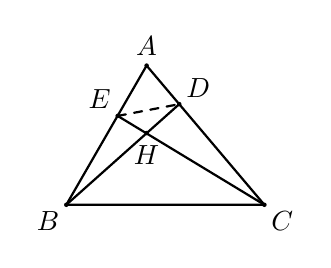
\begin{tikzpicture}[scale=0.68, >=stealth, line join=round, line cap=round]
  \coordinate (A) at (0, 2.6);
  \coordinate (B) at (-1.5, 0);
  \coordinate (C) at (2.2, 0);
  \coordinate (D) at (0.61, 1.88);
  \coordinate (E) at (-0.54, 1.66);
  \coordinate (H) at (0, 1.34);
  \draw[thick] (A) -- (B) -- (C) -- cycle;
  \draw[thick] (B) -- (D);
  \draw[thick] (C) -- (E);
  \draw[thick, dashed] (E) -- (D);
  \fill (A) circle (1.2pt) node[above] {$A$};
  \fill (B) circle (1.2pt) node[below left=-1pt] {$B$};
  \fill (C) circle (1.2pt) node[below right=-1pt] {$C$};
  \fill (D) circle (1.2pt) node[above right=-1pt] {$D$};
  \fill (E) circle (1.2pt) node[above left=-1pt] {$E$};
  \fill (H) circle (1.2pt) node[below=1pt] {$H$};
\end{tikzpicture}
\end{minipage}\par
\vspace{0.4mm}
\noindent\textit{Bài giải:}\dongke{17}
\\ \hline
\end{tabularx}
\end{document}
